 
\section{Naudojamas teorinis modelis}

Šiame darbe modelis pasirinktas atsižvelgiant į vyksmus netvarkiose organinėse medžiagose, tačiau bandyta neapriboti modelio viena medžiagų klase. Taigi modelyje ir simuliacijos programoje yra įskaitomi difuzijos ir krūvininkų dreifo bei rekombinacijos reiškiniai. Patogiam programos rezultatų lyginimui su photo-CELIV eksperimentais programa naudoja realius eksperimentinius parametrus, o ne normuotus dydžius. Taip pat pradiniai krūvininkų tankiai suskaičiuojami iš šviesos intensyvumo ir sugerties profilio. Modelyje laikoma, jog šviesos impulso trukmė yra daug mažesnė už difuzinės relaksacijos ir krūvininkų rekombinacijos trukmes.
Matematinis modelis yra krūvininkų pasiskirstymo uždavinys, kuriame įskaitant krūvininkų pernašą ir rekombinaciją stebima sistemos laikinė evoliucija. Rezultatas -- teorinė photo-CELIV kinetika. Taip pat gali būti atvaizduojami krūvininkų arba elektrinio lauko pasiskirstymai bandinyje bet kuriuo laiko momentu.

\subsection{Uždavinio diskretizavimas}

Daugelio realių photo-CELIV eksperimentų bandiniai yra “sumuštinio” pavidalo. Tokius bandinius galima redukuoti į vienmates parametrų pasiskirstymo funkcijas. Dėl to šiame darbe bandinys modeliuojamas kaip vienmatė krūvininkų tankio funkcija:
\begin{equation}
\begin{array}{c}
n=n(x)\\
p=p(x)
\end{array}
\end{equation}
Čia \(n,p\) atitinkamai neigiamų krūvininkų ir teigiamų krūvininkų tankis. Taip pat supaprastinome uždavinį teigdami, jog dielektrinė skvarba yra konstanta.
\begin{equation}
\varepsilon(x,E)=\textit{const}
\end{equation}
Modeliuojant skaitmeniškai būtina tolydinį tankių pasiskirstymą suskaidyti į diskretinį. Tai atlikta visą bandinį sudalinus į \(M\) narvelių kuriuose krūvininkų kiekis būtų lygus:
\begin{equation}
\begin{array}{c}
N_i = \frac { n(x_i) + n(x_i+1)}{2} \Delta x S\\
P_i = \frac { p(x_i) + p(x_i+1)}{2} \Delta x S
\end{array}
\end{equation}
Čia \(x_i=x i\), kur \(i \in [0,M)\) narvelio numeris, \(x\) narvelio plotis,\(S\) bandinio plotas (žr. \ref{fig:diskretizavimas}~pav.).
\begin{figure}
  \centering
    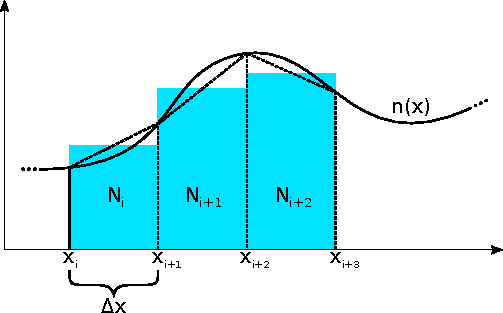
\includegraphics[scale=0.9]{./media/pdf/il1}
  \caption{Tankio diskretizavimas}
  \label{fig:diskretizavimas}
\end{figure}

Diskretizavimas visada įneša netikslumų, tačiau, didindami sudalinimų skaičių \(M\) galime pasiekti norimą skaičiavimo tikslumą (vėliau parodysime, kaip nuo \(M\) priklauso uždavinio trukmė).
Skaičiuojama laikinė sistemos evoliucija, tad reikalingas ir laiko diskretizavimas:
\begin{equation}
\begin{array}{c}
N_i = N_i(t_j) \equiv N_{i,j}\\
P_i = P_i(t_j) \equiv P_{i,j}\\
t_j = t_{j-1} + \Delta t_j
\end{array}
\end{equation}
Čia \(j\) - yra simuliacijos žingsnis, \(\Delta t_j\) - kintamas laiko žingsnis, \(t_j\) diskretizuoto laiko momentas, priklausantis nuo kintamo laiko žingsnio.

\subsection{Dreifas}

Modelyje krūvininkų pernaša vyksta dėl dreifo ir difuzijos. Dreifas skaičiuojamas naudojantis Drūdės modeliu \cite{ashcroft}, kuris teigia, jog esant elektriniam laukui kietajame kūne krūvininkai juda greičiu proporcingu lauko stipriui. Šis greitis vadinamas dreifo greičiu \(v_d\).
\begin{equation}
	v_d= \mu E
\end{equation}
	
Čia \(\mu\) krūvininkų judris, \(E\) elektrinio lauko stipris.
Naudojantis greičio išraiška galime užrašyti srovės tankį:
\begin{equation} \label{eq:tankis}
	j_d = v_d n e = \mu n e E
\end{equation}
Iš kitos pusės, pagal apibrėžimą laikydamiesi anksčiau aprašyto diskretizavimo, srovės tankį galime užrašyti taip:
\begin{equation} \label{eq:pokytis}
\frac{\Delta N_{i,j}}{\Delta t_j} \frac{e}{S}=(j_d)_{i,j}
\end{equation}
	
Krūvininkai, išėję iš narvelio per laiko žingsnį \(\Delta t_j\) sukuria srovę. Nuo krūvininkų ženklo ir išėjimo krypties priklauso sukurtos srovės kryptis. Simuliacijos metu laikoma, jog teigiamą srovę sukuria neigiami krūvininkai judantys koordinatės indekso i didėjimo kryptimi.
Taigi suminis srovės tankis laiko momentu \(t_j\) yra toks:
\begin{equation}
j_d(t_j)= \sum_{i=0}^{M} (j_d)_{i,j}
\end{equation}
	

Naudodamiesi diskretizuota \eqref{eq:pokytis} išraiška ir srovės tankio \eqref{eq:tankis} išraiška galime užrašyti:
\begin{equation}
\frac{\Delta N_{i,j}}{\Delta t_j} = \frac{\mu N_{i,j} E_j}{\Delta x}
\end{equation}
Tuo tarpu elektrinis laukas bandinyje susideda iš išorinio ir vidinio elektrinių laukų:
\begin{equation}
\vec{E} = \vec{E}_{in} + \vec{E}_{ex}
\end{equation}

Mūsų nagrinėjamu atveju išorinį elektrinį lauką kuria įtampa prijungta prie bandinio kontaktų, taigi jį galima laikyti nepriklausoma laikine funkcija:
\begin{equation}
	E_{ex}=f(t)
\end{equation}
Vidinio lauko stipris turi būti apskaičiuojamas naudojant Puasono lygtį:
\begin{equation}
	E_{in}(x)=-\frac{e}{\varepsilon \varepsilon_0 S} \int_{0}^{x} x(n-p)dx
\end{equation}
Matome, jog vidinis elektrinis laukas paverčia nagrinėjamą problemą į integro-diferencialinę lygtį.
Pereiname prie diskretizavimo:
\begin{equation}
	E_{in,i}=-\frac{e}{\varepsilon \varepsilon_0 S } \sum_{k=0}^{i}(N_k-P_k)
\end{equation}
Čia \(E_{in,i}\) lauko stipris kuriamas \(i\)-tojo narvelio.



\subsection{Difuzija}

Esant krūvininkų tankio erdviniam pasiskirstymui, vyksta krūvininkų difuzinė pernaša. Pagal Fiko dėsnį:
\begin{equation}
	\frac{\partial n}{\partial t}=-D \frac{\partial^2 n}{\partial x^2}
\end{equation}
Čia \(D\) difuzijos konstanta.

Krūvininkų tankio antrą išvestinę pagal koordinatę keičiame į gretimų narvelių krūvininkų skaičiaus skirtumą:
\begin{equation} \label{eq:difuzija}
\frac{\Delta N_{i,j}}{\Delta t_j} = -D \frac{(N_{i,j-1}-N_{i-1,j-1})}{(\Delta x)^2} - D \frac{(N_{i,j-1}-N_{i+1,j-1})}{(\Delta x)^2}
\end{equation}
Šiame modelyje naudojamės Einšteino sąryšiu:
\[
	D=\frac{k_B T \mu }{e}
\]	
Formulėje~\eqref{eq:difuzija} užrašyti du nariai norint atskirti krūvininkus judančius tarp \(N_{i-1}\) ir \(N_i\) narvelių, bei krūvininkus judančius tarp \(N_i\) ir \(N_{i+1}\) narvelių. Taip atskirta nes, skirtingai nuo dreifo, vieno ženklo krūvininkai gali išeiti abiem kryptimis.
Kadangi formulė \eqref{eq:difuzija} aprašo bendrą krūvininkų skaičiaus kitimą narvelyje dėl difuzijos, sumuojant difuzinę srovę naudojamas tik teigiamas pokytis, tai yra, norint išvengti dvigubos sumos, sumuojami tik iš narvelio išeinantys krūvininkai. Sumavimas analogiškas dreifo srovės komponentės skaičiavimui:
\begin{equation}
	\frac{\Delta N_{i,j}}{\Delta t_j} \frac{e}{S}=(j_c)_{i,j}
\end{equation}
\begin{equation}
	j_c(t_j)= \sum_{i=0}^{M} (j_c)_{i,j}
\end{equation}
	
\subsection{Rekombinacija}

Kietajame kūne egzistuoja keli krūvininkų rekombinacijos mechanizmai, pavyzdžiui monomolekulinė rekombinacija, bimolekulinė ar trimolekulinė (Ožė) rekombinacija. Organiniuose puslaidininkiuose monomolekulinė rekombinacija vyksta, kai judantį krūvininką pagauna rekombinacijos centras. Toks mechanizmas priklauso tik nuo vienų krūvininkų tankio, laikant jog centrų kiekis yra daug didesnis ir nekinta vykstant rekombinacijai. Tuo tarpu esant palyginamiems abiejų ženklų krūvininkų tankiams arba kai krūvininkai juda nestipriame potenciniame lauke, rekombinacijos sparta ima priklausyti nuo abiejų ženklų krūvininkų tankių. Būtent tokios sąlygos pasirinktos aprašomame modelyje. Organinėse medžiagose bimolekulinę rekombinaciją lemia dar ir tai, kad pernaša vyksta šuoliais arba krūvininkams tuneliuojant per tarpmolekulinius barjerus. Kitaip tariant krūvininkai yra priversti kurį laiką būti lokalizuoti ties viena molekule, ir tuo metu gali rekombinuoti su kitu atėjusiu krūvininku. Trimolekulinė rekombinacija yra nežymi organiniuose puslaidininkiuose, taigi jos galime nepaisyti \cite{juška:143303,juška:013303}.
Remiantis Lanževeno \cite{langevin} aptartu atveju, efektinė bimolekulinės rekombinacijos sparta yra propocinga krūvinkų judriui:
\begin{equation}
B_L=\frac{e}{\varepsilon \varepsilon_0}(\mu_n+\mu_p)
\end{equation}
Taigi rekombinacijos spartą galime aprašyti taip:
\begin{equation} \label{eq:langevin}
\frac{dn}{dt}=-B_L n p
\end{equation}
Tačiau dažnai eksperimentuose stebimas rekombinacijos spartos neatitikimas su Lanževeno teorine verte \(B_L\). Išmatuota rekombinacijos sparta būna mažesnė už teorinę \cite{juška:155202}. Dėl šio neatitikimo į \eqref{eq:langevin} formulę įvedamas redukcijos faktorius \(\eta\), parodantis kiek kartų rekombinacija silpnesnė už teorinę:
\begin{equation}
	\frac{dn}{dt}=-\eta B_L n p
\end{equation}
Kai kuriais atvejais šis rekombinacijos susilpnėjimas yra naudingas, pavyzdžiui, saulės elementų gamyboje, kur norima naudoti medžiagas su dideliu judriu, tačiau silpna rekombinacija.
Rekombinacijos sparta simuliacijoje valdoma keičiant valdantį parametrą \(\eta\).

\subsection{Šviesos sugertis}

Krūvininkų sukūrimui photo-CELIV metodikoje naudojamas šviesos impulsas. Dėl to pradinis krūvininkų pasiskirstymas yra apskaičiuojamas pagal Beer-Lambert’o taisyklę šviesos sugerčiai:
\begin{equation}
	I(x)=I_0 e^{-\alpha x}
\end{equation}
Čia \(I_0\) šviesos intensyvumas ties bandinio paviršiumi, \(I(x)\) šviesos intensyvumas gylyje \(x\), \(\alpha\) sugerties koeficientas.
Simuliacijoje laikome jog apšviečiama bandinio \(x=0\) ploštuma.

Dažnai vietoje \(\alpha\) naudojamas sugerties profilio parametras \(\alpha d\) kuris priklausomai nuo skaitinės vertės leidžia įvardinti sugerties tipą: \(\alpha d < 1\) sugertis tūrinė, krūvininkai sukuriami beveik vienodai visame tūryje, \(\alpha d > 1\) sugertis paviršinė, beveik visa šviesa sugeriama bandinio paviršiuje. Čia \(d\) yra bandinio storis.
Laikydami, jog generacijos kvantinis našumas yra lygus vienetui, tai yra, jog vienas fotonas sukuria vieną porą krūvininkų, galime užrašyti pradinį generuotų krūvininkų skaičių:
\begin{equation}
	P_0(x) = N_0(x) = I(x)S
\end{equation}
	
Čia \(I(x)S\) yra poras kuriančių fotonų skaičius gylyje \(x\).
Taigi pradinės sąlygos priklauso nuo dviejų parametrų: \(I_0\) (šviesos intensyvumo) ir \(\alpha d\) (sugerties profilio). Ankstesniuose skaičiavimuose buvo parodyta šių parametrų įtaka photo-CELIV signalui \cite{juška:155202}.

Programoje generuojamų krūvininkų kiekis valdomas keičiant parametrą \(I_0 S\).